\section{Toy example}
We can now look at the toy example from the notebook and slides. We define $u(x,y): \mathbb{R}^2 \rightarrow \mathbb{R}$ and we define the partial differential equation:
\begin{equation}
	f(x,y) = \nabla^2 u - \kappa^2 u = \frac{\partial^2 u}{\partial x^2} + \frac{\partial^2 u}{\partial y^2} + \kappa^2 u \label{eq:4}
\end{equation}
Where \textit{f} is known to us. As \textit{u} is unknown we need a way to simplify the partial derivatives in \autoref{eq:4}. This is where our finite difference approximations comes into the picture. Using (for instance) the central difference approximation we can now approximate the partial derivatives in terms of the surrounding nodes in our sampled grid. Using central difference approximation we can thus simplify \autoref{eq:4} to:
\begin{align*}
	f_{i,j} &= \frac{u_{i+1,j} - 2u_{i,j} + u_{i-1,j}}{\Delta x^2} + \frac{u_{i,j+1} - 2u_{i,j} + u_{i,j-1}}{\Delta y^2} - \kappa^2 u\\
	&= \frac{1}{\Delta x^2}u_{i-1,j} + \frac{1}{\Delta y^2}u_{i,j-1} + \left(-\kappa^2 - \frac{2}{\Delta x^2} - \frac{2}{\Delta y^2}\right)u_{i,j} \\
	&\quad + \frac{1}{\Delta y^2}u_{i,j+1} + \frac{1}{\Delta x^2}u_{i+1,j}
\end{align*}
If we now substitute all the coefficients before the \textit{u} terms with $c's$ (to shorten / generalize notation) we can derive \textit{update formulas} for the \textit{u} terms. We can for instance derive the update formula for the unknown $u_{i,j}$ as:
\begin{equation*}
	u_{i,j} = \frac{f_{i,k} - c_{i-1,j}u_{i-1,j} - c_{i,j-1}u_{i,j-1} - c_{i,j+1}u_{i,j+1} - c_{i+1,j}u_{i+1,j}}{c_{i,j}}
\end{equation*}
We here refer to \textit{f} as the \textit{source term}. From the update formula of $u_{i,j}$ we see which other \textit{u} terms $u_{i,j}$ depends on. We can visualize this in terms of a \textit{stencil} which more visually gives a notion of which other nodes in our grid our nodes depend on.
\begin{figure}[H]
	\centering
	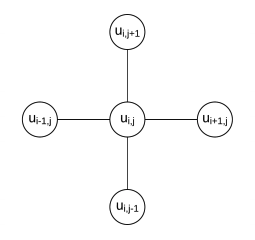
\includegraphics[width=0.4\linewidth]{Materials/stencil}
	\caption{Visualization of a stencil. Illustration taken from lecture slides.}
	\label{stencil}
\end{figure}
In \autoref{stencil} we can see an illustration of a stencil. We can imagine running this stencil over each node in our grid, which would then gives us the update formula for each node in the grid in terms of dependent nodes. However, we quickly realize that the stencil would stick outside our grid at the boundaries. We thus need some boundary conditions to handle what should happen at the boundaries. 

\subsection{Boundaries}
\begin{figure}[H]
	\centering
	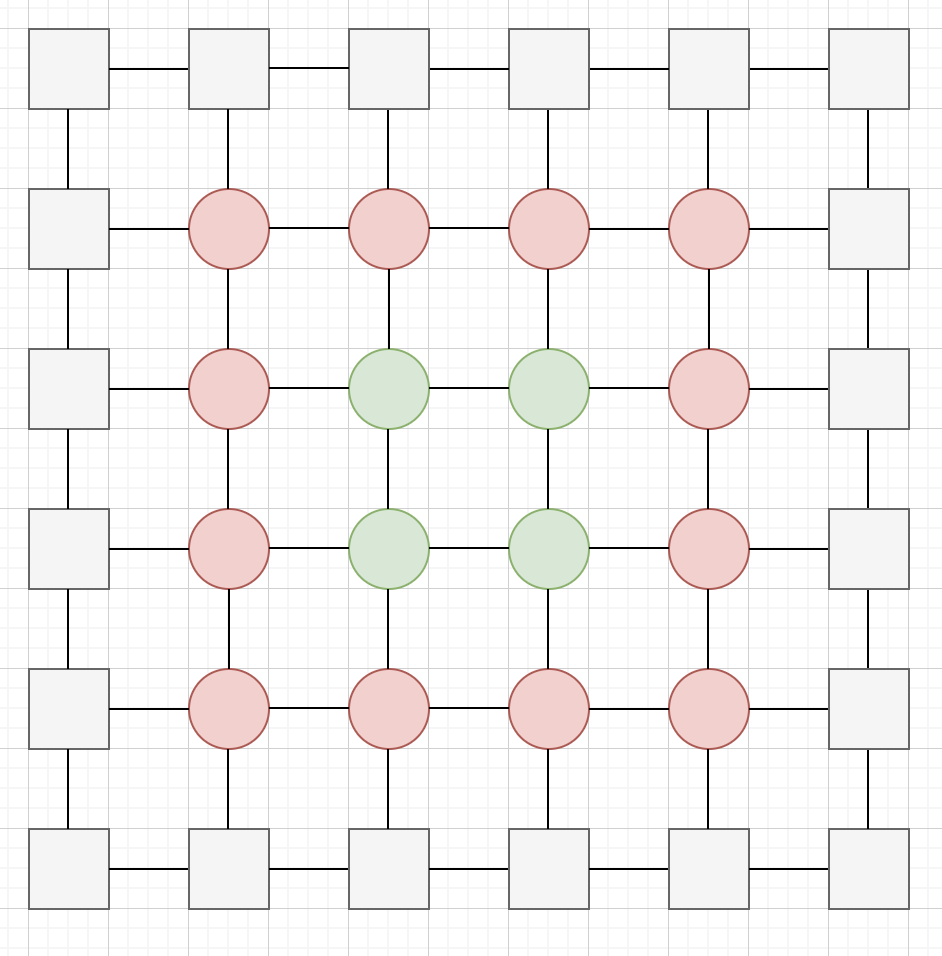
\includegraphics[width=0.3\linewidth]{Materials/grid}
	\caption{Visualization of a grid with the green and red circles being domain nodes, red circles being boundary nodes and the square nodes being ghost nodes..}
	\label{grid}
\end{figure}
Two common boundary conditions are Dirichlet and von Neumann boundary conditions. We define them as:
\begin{align*}
	u(x,y) &= k_d, \quad \forall x,y \in \Gamma\\
	\frac{\partial u}{\partial x} &= k_n, \quad \forall x,y \in \Gamma
\end{align*}
Where $\Gamma$ is the 'boundary of the boundary nodes' (the boundary nodes can be seen in \autoref{grid}). We can apply one of two techniques to deal with boundary conditions, we either use elimination of unknown variables or we use ghost nodes. If we choose to apply a von Neumann boundary condition and we choose to apply elimination of variables to handle it, then for the left side of the grid, using central difference approximations, we will have:
\begin{align*}
	\frac{\partial^2 u_{1,j}}{\partial x^2} &= \frac{\frac{\partial}{\partial x}u_{\frac{1}{2},j} - \frac{u_{2,j} - u_{1,j}}{\Delta x}}{\Delta x}\\
	&= \frac{u_{1,j} - u_{2,j}}{\Delta x^2}
\end{align*}
As $\frac{\partial}{\partial x}u_{\frac{1}{2},j}$ is zero according to the von Neumann boundary condition. That is, we can compute the left boundary conditions as a negative forward difference approximation. Similarly, if $x_i = 5$ is our right boundary we have for the right boundary conditions:
\begin{align*}
	\frac{\partial^2 u_{5,j}}{\partial x^2} &= \frac{\frac{u_{5,j} - u_{4,j}}{\Delta x} - \frac{\partial}{\partial x}u_{5\frac{1}{2},j}}{\Delta x}\\
	&= \frac{u_{5,j} - u_{4,j}}{\Delta x^2}
\end{align*}
Which is a backwards difference approximation. This also extends symmetrically to the top and bottom boundary conditions.\\
If we choose to use the ghost node approach we then extends our grid. This can be seen in \autoref{grid} where the circles is our domain and the squares are 'extra' nodes which we append to ensure the stencil never goes out of bounds. To find the values of these ghost nodes we can now 'unpack' the von Neumann boundary conditions from above:
\begin{equation*}
	\frac{\partial}{\partial x}u_{\frac{1}{2},j} = \frac{u_{1,j} - u_{o,j}}{\Delta x} = 0
\end{equation*}
This implies $u_{0,j} = u_{1,j}$ (we would obtain similar results if we looked at the other boundaries), that is our boundaries should 'reflect' or mirror the domain values it is 'facing'. 

\subsection{Solutions}
Now that we have dealt with our boundaries, we can compute solutions in two different ways. First we can use our stencil, and iteratively go over all domain nodes in our grid updating each node according to our update formula. This requires we make an initial guess for the values of our nodes which simply could be all of them are equal to zero at iteration zero. We would keep updating our nodes until they 'converge', i.e. the nodes no longer change.\\
Another way to compute a solution is to note the stencils form linear systems of equations where we have:
\begin{align*}
	f_{1,1} &= c_{1,0}u_{1,0} + c_{0,1}u_{0,1} + c_{1,1}u_{1,1} + c_{2,1}u_{2,1} + c_{1,2}u_{1,2}\\
	&\vdots \\
	f_{n-1,m-1} & = c_{n-1,m-2}u_{n-1,m-2} + c_{n-2,m-1}u_{n-2,m-1}\\
	&\quad + c_{n-1,m-1}u_{n-1,m-1} + c_{n,m-1}u_{n,m-1} + c_{n-1,m}u_{n-1,m}
\end{align*}
Where \textit{n} and \textit{m} are the size of the grid. We can similarly write a linear system for the boundary conditions. If we split the coefficients and the \textit{u} values we can construct the matrix system $\mathbf{Au} = \mathbf{f}$ where \textbf{A} encodes the coefficients and \textbf{f} is our vectorized grid values. We can compute the vector index from the 2d grid indices as $k = jN+i$ where \textit{N} is the number of columns in the grid. To construct \textbf{A} we similarly use the encoding $\mathbf{A}_{(jN+i),(bN+a)} = c_{a,b}$ where we would define \textit{a} and \textit{b} in relation to \textit{i} and \textit{j}, i.e. if we want to encode the middle node of our stencil, this would have index $\mathbf{A}_{jN+i),jN+i)}$ and the left arm of the stencil would have index $\mathbf{A}_{jN+i),((j-1)N+i)}$. This maps our stencils to rows of \textbf{A} as seen in \autoref{stencilencoding}. After the encoding we can simply solve $\mathbf{Au} = \mathbf{f}$ for \textbf{u}. This process is called \textit{matrix assembly}.
\begin{figure}[H]
	\centering
	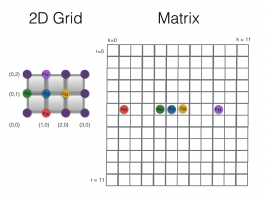
\includegraphics[width=0.5\linewidth]{Materials/stencilencoding}
	\caption{Visualization of a grid with the green and red circles being domain nodes, red circles being boundary nodes and the square nodes being ghost nodes.}
	\label{stencilencoding}
\end{figure}